\documentclass[a4paper,12pt,fleqn]{article} % добавить leqno в [] для нумерации слева

%%% Работа с русским языком
\usepackage{cmap}					% поиск в PDF
\usepackage{mathtext} 				% русские буквы в формулах
\usepackage[T2A]{fontenc}			% кодировка
\usepackage[utf8]{inputenc}			% кодировка исходного текста
\usepackage[english,russian]{babel}	% локализация и переносы

%%% Дополнительная работа с математикой
\usepackage{amsmath,amsfonts,amssymb,amsthm,mathtools} % AMS
\usepackage{icomma} % "Умная" запятая: $0,2$ --- число, $0, 2$ --- перечисление

%% Номера формул
%\mathtoolsset{showonlyrefs=true} % Показывать номера только у тех формул, на которые есть \eqref{} в тексте.

%% Шрифты
\usepackage{euscript}	 % Шрифт Евклид
\usepackage{mathrsfs} % Красивый матшрифт
%\usepackage[fleqn]{amsmath}

%% Свои команды
\DeclareMathOperator{\sgnL}{\mathop{sGgn}}

%% Перенос знаков в формулах (по Львовскому)
\newcommand{\hm}[1]{#1\nobreak\discretionary{}
{\hbox{$\mathsurround=0pt #1$}}{}}

\newenvironment{changemargin}[2]{%
\begin{list}{}{%
\setlength{\topsep}{0pt}%
\setlength{\leftmargin}{#1}%
\setlength{\rightmargin}{#2}%
\setlength{\listparindent}{\parindent}%
\setlength{\itemindent}{\parindent}%
\setlength{\parsep}{\parskip}%
}%
\item[]}{\end{list}}

\begin{document} % конец преамбулы, начало документа
\section{Состав и обязанности разработчиков}
\begin{itemize}
    \item Волков В.Д.
        \begin{itemize}
            \item построение основной структуры программы
            \item механизмы обработки событий игры на глубинном, не GUI, уровне
            \item часть вспомогательных функций
        \end{itemize}
    \item Иртикеев М.Н.
        \begin{itemize}
            \item обработка событий игры на GUI уровне
            \item создание интерфейса для корректной работы игры
        \end{itemize}
    \item Гуняшов Н.Н.
        \begin{itemize}
            \item разработка режима сетевой игры
            \item создание игрового редактора юнитов
        \end{itemize}
\end{itemize}

\newpage
\section{Постановка задачи}
В качестве объекта нашей работы мы решили выбрать стратегию реального времени.
Основными критериями нашего выбора являются:
\begin{itemize}
    \item Возможность объединить множество аспектов программирования в рамках одной программы.
    \item Возможность работать в коллективе ( одно из важнейших качеств программиста ), при этом не испытывая проблем с разделением труда и совместной разработкой.
    \item Приятное и не требующее особых навыков тестирование.
    \item Возможность почти неограниченного усложнения функционала ( в случае наличия времени можно сделать свой игровой движок, искусственный интеллект или игру по сети и т.д. ). 
    \item Легко найти тестеров, что несомненно может быть важно для некоторых аспектов ( в частности игре по сети ).
\end{itemize}
\newpage

\section{Методы разработки}
Основными методами, выбранными нами при разработке являются \textbf{классы} и \textbf{наследование}.
Также как технологические решения можно выделить большое количество элементов типа \textbf{std::list},
 которые используются для быстрого удаления элементов,
 а невозможность быстрого доступа по индексу(итератору) компенсируется частым использованием \textbf{указателей}.
 Использование ссылок оказалось затруднительным в связи с невозможностью std::vector<\&объект> и std::list<\&объект>.
 Все \textbf{юниты}, \textbf{здания} и \textbf{прочие типы объектов} являются объектами, а не классами,
 что позволяет сделать удобный \textbf{редактор}, в котором пользователям можно будет создавать свои игровые единицы. 
Прототипы игровых единиц хранятся в \textbf{std::vector} прототипов для юнитов,
 зданий и прочих классов в классе Game, откуда для нужд игроков будут делаться играбельные ``слепки''.

Также можно отметить что многие алгоритмы в игре будут связаны с \textbf{графами} и поэтому
 будет много \textbf{обходов графов в ширину}, \textbf{определение кратчайшего расстояния между вершинами}
 и прочих алгоритмов из теории графов.

\newpage
\section{Выбор языка разработки}
Выбор пал на язык с++, так как он даёт:
\begin{itemize}
    \item возможность работать как на высоком, так и на низком уровне
    \item понятен большинству программистов
    \item позволяет легко реализовать возможности ООП
    \item имеет множество полезных для разработки данного проекта библиотек
    \item имеет высокую скорость работы по сравнению со многими другими языками
    \item является компилирующимся языком, что усилит быстродействие игры
\end{itemize}

\newpage
\section{Выбор других средств разработки}
\begin{itemize}
    \item операционные системы: GNU/Linux Arch, Windows 10
    \item система контроля версий: Git
    \item система компьютерной верстки: TeX (LaTeX)
\end{itemize}

\newpage
\section{Структура}
Создана посредством импорта в umbrello5 текущего кода

\begin{changemargin}{-3cm}{-2cm}
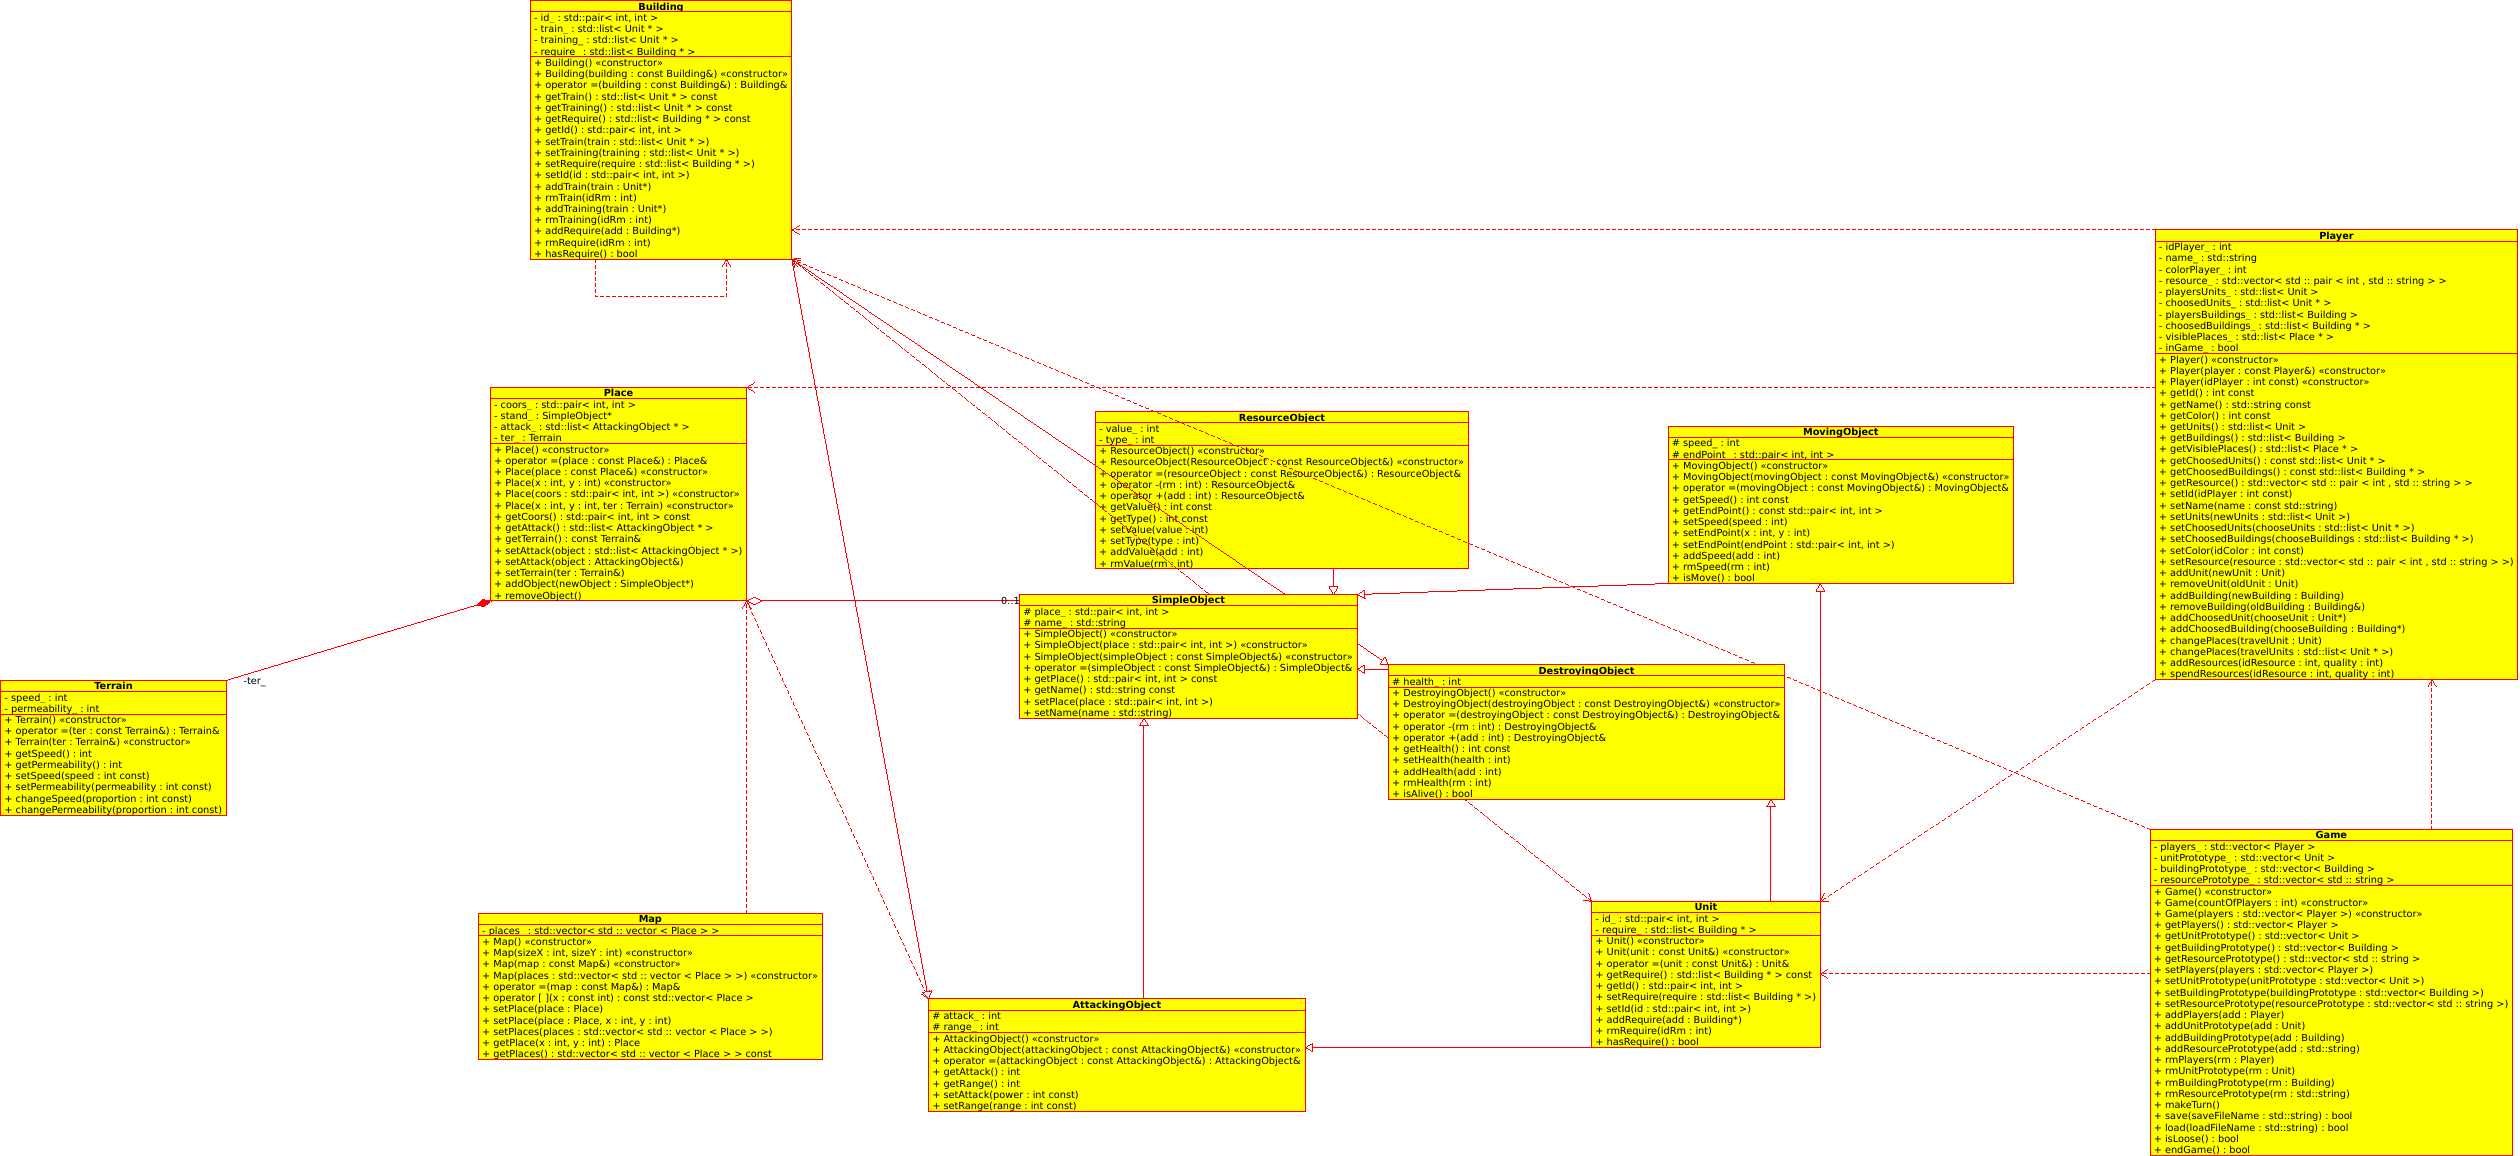
\includegraphics[width=1\linewidth]{structure}
\end{changemargin}
* методы в классах могут меняться в процессе разработки, также вероятно изменятся некоторые не очевидные названия
%** граф не планарен, поэтому без пересечений в 2D-мерном пространстве отобразить не получится

\end{document} % конец документа

